% TODO:
%   - Kijk na of titels in header overflowen
% ----------  
% Questions:
%   - XXX


% In a new chapter, reset the GLS to once again use full version in first occurence
\glsresetall

\chapter{Decoding brain signals with machine learning}
\label{ch:processing_signals}

% ---------------------------------------------- 
% INTRODUCTION
% ---------------------------------------------- 
\section{Introduction to this chapter}
\label{sec:processing_signals_introduction}
% NOTE: "Introduction" exists in each chapter and gives short intro to chapter + what can be expected in chapter

The previous chapter, Chapter \ref{ch:biomedical_signals} discussed \gls{biosignal} and how bioelectricity is made in the human body.
Multiple modalities for measuring brain signals were discussed and it was discussed how \gls{eeg} seems like the most promising measuring modality for capturing \gls{elecbiosignal} from the brain in a \gls{bci} setting.
Chapter \ref{ch:biomedical_signals} also discussed that \gls{mi} is one of many methods to induce such \gls{elecbiosignal} activity in the brain, namely by causing \gls{ers} and \gls{erd}.
\gls{mi} and \gls{ers}/\gls{erd} were deemed interesting as it doesn't require the external stimuli that \gls{ep} do and applies to many people, even those with limited mobility.
However, it was also discussed that \gls{ers}/\gls{erd} following from methods such as \gls{mi} require extensive user training and are harder to detect than most \gls{ep} alternatives for inducing such \gls{elecbiosignal} activity in the brain.

This chapter will discuss how brain signals can be decoded using both traditional two-step \gls{ml} and one-step \gls{dl} in more detail.
Whilst Chapter \ref{ch:bci} already highlighted multiple breakthroughs in this regard on an intuitive level, this chapter will provide more technical details.
First, the general pipeline for classifying brain signals and \gls{mi} \gls{eeg} in particular is discussed.
Then the role of \gls{ml} and \gls{dl} in this pipeline and some of the most important concepts from these technologies are discussed.
This chapter then goes over the process of evaluating and using the created and trained pipelines.
The chapter concludes by discussing some of the common issues encountered while creating these pipelines and the conclusions that can be made from this chapter.


% ---------------------------------------------- 
% GENERAL TRAINING PIPELINE
% ---------------------------------------------- 
\section{A general pipeline for classifying brain signals}
\label{sec:processing_signals_general_pipeline}

\begin{sidewaysfigure}
    \centering
    \begin{subfigure}{\textwidth}
        \centering
        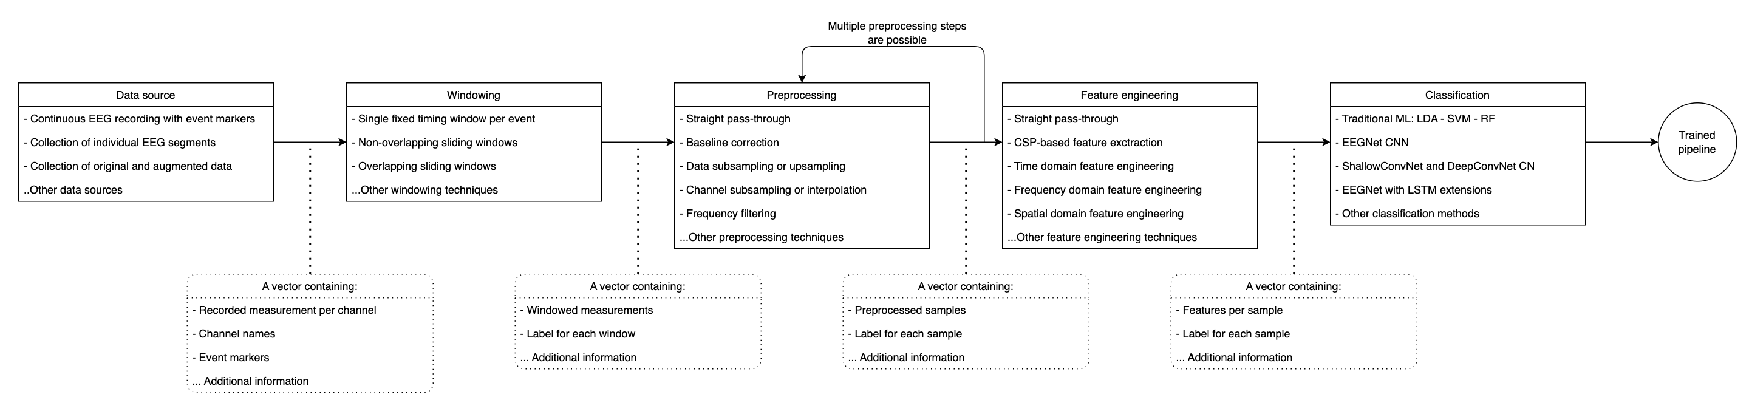
\includegraphics[width=\textwidth]{../images/pipeline/brain_signal_pipeline_training.pdf}
        \captionsetup{width=0.9\linewidth}
        \captionsetup{justification=centering}
        \caption{Components of general training pipeline for brain signal classification annotated with common examples per component.}
        \label{fig:processing_signals_pipeline_ml}
    \end{subfigure}
    \hfill
    \begin{subfigure}{\textwidth}
        \centering
        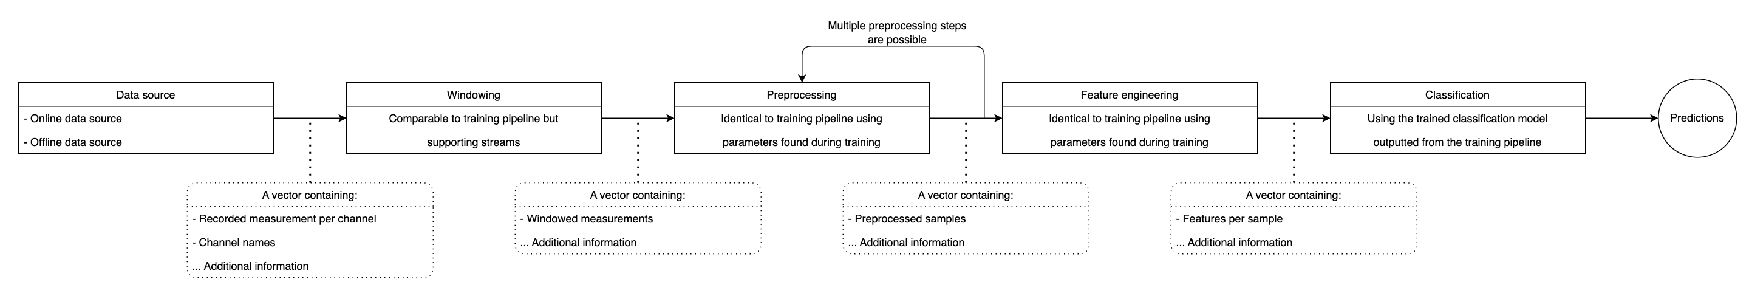
\includegraphics[width=\textwidth]{../images/pipeline/brain_signal_pipeline_predicting.pdf}
        \captionsetup{width=0.9\linewidth}
        \captionsetup{justification=centering}
        \caption{Components of general prediction pipeline for brain signal classification annotated with common examples per component.}
        \label{fig:processing_signals_pipeline_dl}
    \end{subfigure}
    \captionsetup{width=0.9\linewidth}
    \captionsetup{justification=centering}
    \caption{General training pipeline and prediction pipeline used for classifying brain signals.}
    \label{fig:processing_signals_pipeline}
\end{sidewaysfigure}

The general pipeline of classifying brain signals and \gls{eeg}-based \gls{mi} tasks in particular is similar to that of a \gls{cad} systems which was discussed in Section \ref{subsubsec:bci_gaining_popularity_improved_data_processing_better_ml_dl} and shown in Figure \ref{fig:cad_pipeline}.
Whilst the training pipeline and prediction pipeline for classifying brain signals consist of the same components, their input and output are different.
For this reason, this master thesis considers them as two separate pipelines.
The remainder of this section will discuss the components used in these brain signal classification pipelines and the techniques commonly used in each of these components.
Figure \ref{fig:processing_signals_pipeline} provides a visual overview of these pipelines and their components.

% - - - - - - - - - -
% Data acquisition
% - - - - - - - - - -

\subsection{Data source}
\label{subsec:processing_signals_general_pipeline_data_acquisition}

% duidelijk bespreken welk ding echt CS en welk ding eigenlijk derden
% Bespreken data truc * 100xxx voor volt (of al besproken?)

Assuming supervised learning, a \gls{ml} paradigm further discussed in Section \ref{subsec:processing_signals_ml_and_dl_tyes_of_learning_supervision}, input data for the training pipelines should include both the independent variables as wel the dependent variable.
When working with an \gls{eeg} \gls{mi} classification problem, these independent variables are the \gls{eeg} measurements of each channel whilst the dependent variable is the \gls{mi} task performed at a specific time point.
Multiple possibilities exist for providing these variables and the link between them.
Most open-source \gls{mi} \gls{eeg} datasets, such as the one by \citet{eeg_data} used in this master thesis, do this by providing the \gls{eeg} recordings of an entire session as a single 2D matrix (channels x measurement per time point) and the desired labels as an equal width vector containing the marker at any given time point.
The time points are dependent on the sampling frequency and denote the sample number counting from the first sample of the session.
The marker may be the current content of the screen which provides tasks to the user or other event-related information.
Figure \ref{fig:processing_signals_data_source_eeg} combines both the independent and dependent variables into a singular visualisation.

The prediction pipeline only expects the independent variables as its task is to predict the dependent variable.
In theory, these independent variables should be of the same format used during training, but in practice, they might originate from a different source or recording and as such might require additional steps during preprocessing to ensure at least an equal sampling frequency and channel distribution.
This master thesis assumes the device used during training and prediction is identical with equal settings used and as such doesn't require this type of preprocessing.

The prediction pipeline may work in an offline manner, as is the case for the experiments in this master thesis, or in an online manner.
When using offline prediction the data was already recorded and stored before being provided in its totality to the prediction pipeline.
In an online setting, the data is streamed to the prediction pipeline as it is being measured and the prediction pipeline should merge this incoming data to an object that is usable in the next stages itself.
For example, a buffer may be used to collect samples until one second is obtained and pass that to the next step.
In an online setting, windowing is often directly performed on the stream, as discussed next.
Other types of data formatting are possible but they should all provide the same information.

\begin{figure}[ht]
    \centering
    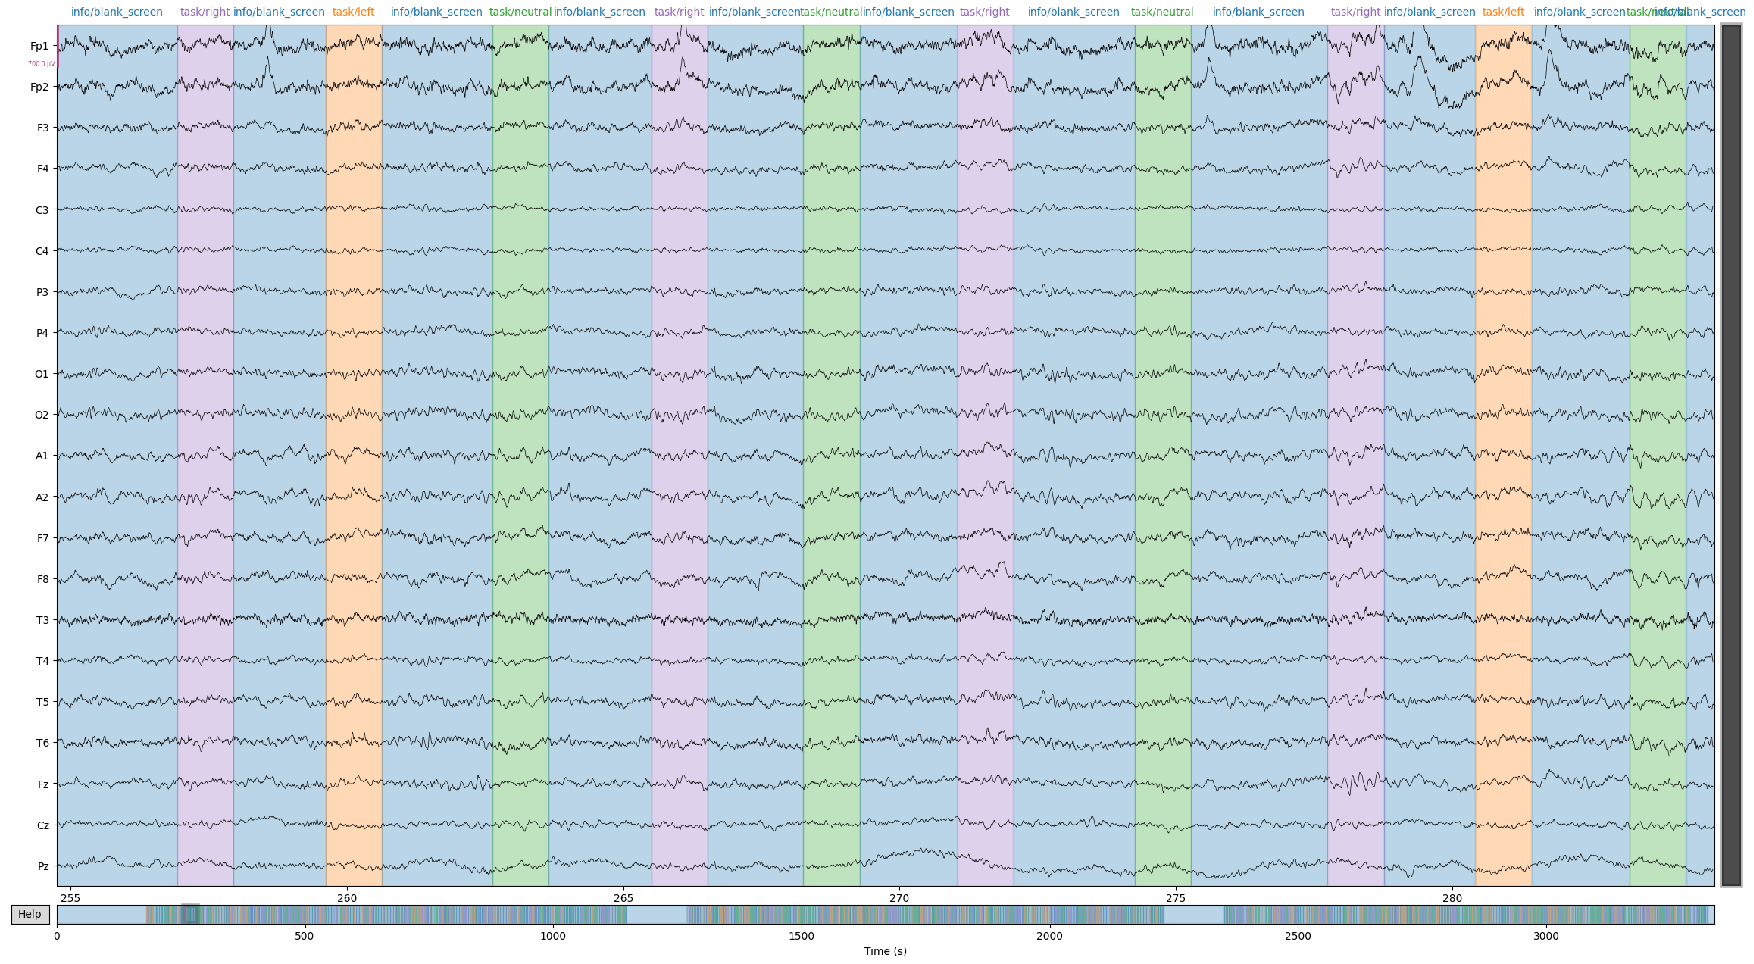
\includegraphics[width=\linewidth]{../images/pipeline/eeg.pdf}
    \captionsetup{width=0.9\linewidth}
    \captionsetup{justification=centering}
    \caption{Visualisation of the \gls{eeg} recording from December 15 2015 overlayed with the provided markers for subject B in the open-source dataset by \citet{eeg_data}. The x-axis depicts the time in seconds, the y-axis depicts which channel of the recording is visualised and the colour overlay represents the active marker.}
    \label{fig:processing_signals_data_source_eeg}
\end{figure}

% - - - - - - - - - -
% Windowing
% - - - - - - - - - -

\subsection{Windowing}
\label{subsec:processing_signals_general_pipeline_windowing}

% Several windowing methods exist and are reviewed by Podder et al (2014).

% Windowing: when specific events in a signal (such as a spike or pattern) matters more than the overall shape of the complete signal, windowing allows to split a signal into fixed-length, usually overlapping, sub-sequences. Having the network focus on small sub-sequences allows it to be faster (less compute intensive, as less data is being processed), and generalize better, as a small number of easily-recognizable patterns (on which the network focuses) can appear in various positions in longer signals (that the network does not have to bother with). Several windowing methods exist, and are reviewed by Podder et al (2014). Jeong et al (2020) and Nguyen and Chung (2019) use Hamming windowing.

The data source as described in Section \ref{subsec:processing_signals_general_pipeline_data_acquisition} provides a continous signal over multiple channels.
To process these signals a mechanism has to be in place so that this continuous signal is split into discrete segments.
Such techniques are often referred to as windowing, but the neurophysiological field also refers to it as epoching.
The latter should not be confused with the meaning of epochs in a \gls{ml} setting.
Different types of windowing exist and three common approaches are illustrated in Figure \ref{fig:processing_signals_windowing}.
Using a fixed window surrounding known event points is trivial on the training data and results in the simplest classification task with the most consistent window labels from the three windowing techniques shown in Figure \ref{fig:processing_signals_windowing}.
However, when trying to predict outcomes, the point at which an event occurs has to be known as well.
This information may be known, for example during an offline \gls{mi} classification task or when using a fixed feedback loop in an online manner where actions from the user are accepted at fixed time intervals.

\begin{figure}[ht]
    \centering
    \begin{subfigure}{0.45\textwidth}
        \centering
        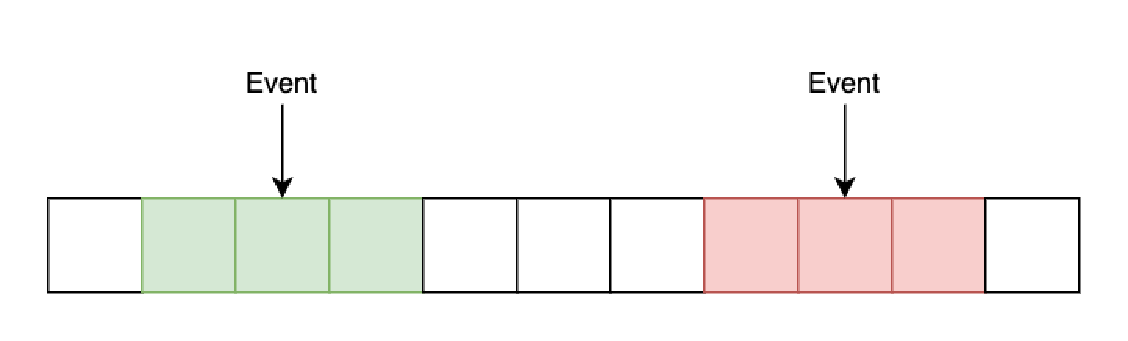
\includegraphics[width=\textwidth]{../images/pipeline/fixed_window.pdf}
        \captionsetup{width=\linewidth}
        \captionsetup{justification=centering}
        \caption{Fixed window surround known event.}
        \label{fig:processing_signals_windowing_non_fixed}
    \end{subfigure}
    \hfill
    \begin{subfigure}{0.45\textwidth}
        \centering
        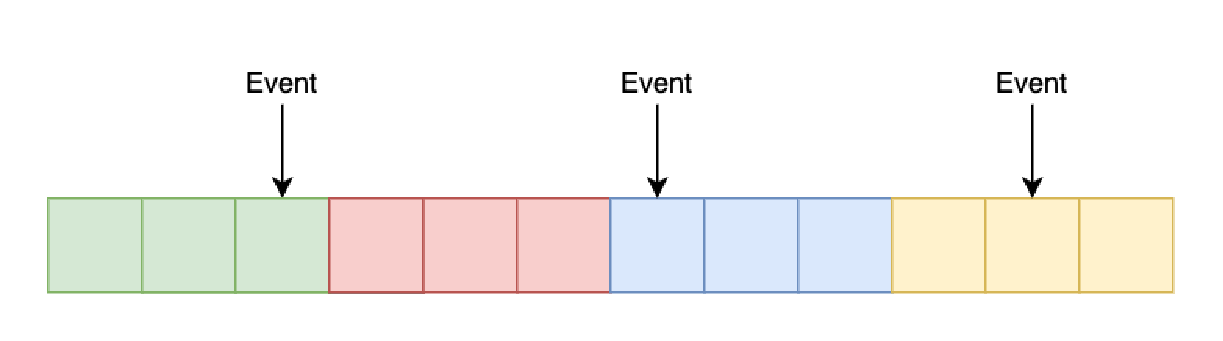
\includegraphics[width=\textwidth]{../images/pipeline/non_overlapping_window.pdf}
        \captionsetup{width=\linewidth}
        \captionsetup{justification=centering}
        \caption{Non-overlapping sliding windows.}
        \label{fig:processing_signals_windowing_non_overlapping}
    \end{subfigure}
    \hfill
    \begin{subfigure}{0.45\textwidth}
        \centering
        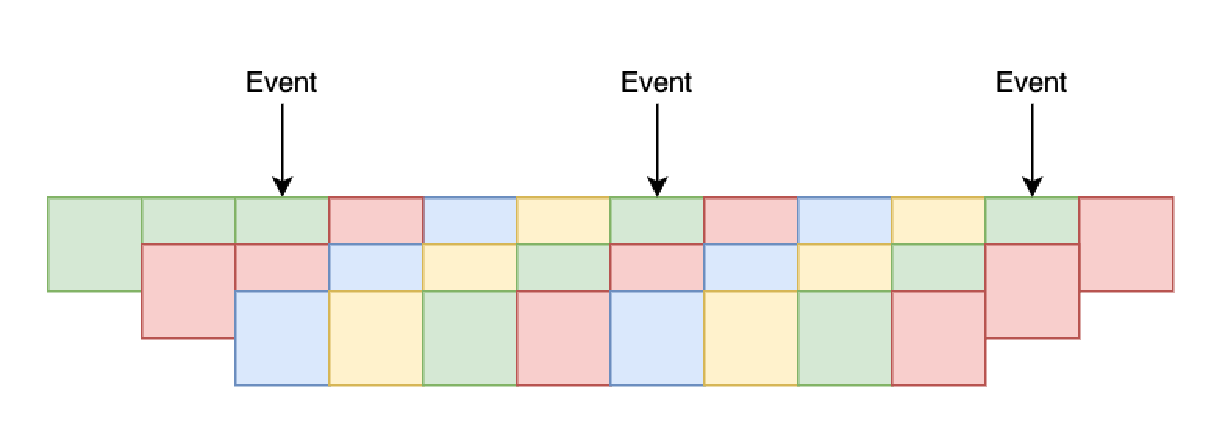
\includegraphics[width=\textwidth]{../images/pipeline/overlapping_window.pdf}
        \captionsetup{width=\linewidth}
        \captionsetup{justification=centering}
        \caption{Overlapping sliding windows}
        \label{fig:processing_signals_windowing_overlapping}
    \end{subfigure}
    \captionsetup{width=\linewidth}
    \captionsetup{justification=centering}
    \caption{Different types of windowing techniques.}
    \label{fig:processing_signals_windowing}
\end{figure}

A more intuitive but computationally harder windowing technique is using sliding windows.
A non-overlapping sliding window technique is shown in Figure \ref{fig:processing_signals_windowing_non_overlapping} and an overlapping technique is shown in Figure \ref{fig:processing_signals_windowing_overlapping}.
Both are trivial to apply to the independent variables but deciding which dependent variable should be related becomes a difficult task.
How much activity from the event should be included for the training window to be considered a sample of that event?
What happens when a window includes two distinct events?
These are questions that should be answered within the context of the application.
When using sliding windows, singular labels such as "task right" may be split into "task right start", "task right hold" and "task right end".

Many different windowing techniques exist that use far more complex strategies than the ones illustrated in Figure \ref{fig:processing_signals_windowing}, especially for controlling the boundaries of the window.
\citet{complex_windowing} discuss some of these more complex windowing techniques in more detail.
When done right, certain sliding window techniques can improve the performance of a \gls{mi} \gls{eeg} classification pipeline compared to even fixed windowing surround a known event, as shown by \citet{sliding_windows_better}.
However, starting a new sliding window at each time point may cause significant computational overhead, increasing both training and prediction time.
The latter can make the prediction pipeline too complex to be run on affordable, low-energy and portable computational hardware as desired by a \gls{bci} system doing local processing.
This master thesis will consider a fixed window of 0.5 seconds and 1.5 seconds surround a known event for both training and prediction.

% - - - - - - - - - -
% Preprocessing
% - - - - - - - - - -

\subsection{Preprocessing}
\label{subsec:processing_signals_general_pipeline_preprocessing}

Brain signals are non-linear as well as non-stationary signals and exact execution of the performed \gls{mi} tasks are bound to differ per subject as already discussed in section \ref{subsec:biomedical_signals_working_with_eeg_generalisation}.
Combining these properties with the poor \gls{snr} of \gls{eeg}, as discussed in Section \ref{tab:biomedical_signals_modalities}, means that raw \gls{eeg} measurements are hard to intepret, even by machines.
Luckily, as discussed by \citet{bci_review_arnau}, a \gls{dl} approach making use of sufficient layer, nodes and training should be capable of learning any mapping from input to output, including any manual preprocessing that can be done.
As such, \gls{dl} approaches can often work directly on this raw \gls{eeg} signal and raw signals in general.
This is one of the most promising aspects of \gls{dl} in multiple fields and it is the reason the one-step \gls{dl} approaches from this master thesis will use no preprocessing besides the \gls{ac} artefact removal that was already performed by the suppliers of the open-source database \citep{eeg_data}.
Traditional two-step \gls{ml} approaches do not have this property of being able to learn any mapping from input to output and as such require at least minimal preprocessing of the data to obtain usable results.
For this reason, many libraries providing the most basic \gls{eeg} preprocessing steps have been developed with MNE by \citet{mne} being the most popular for Python and used in this master thesis.
Some automated pipelines specifically for \gls{eeg} preprocessing have also been proposed, such as the PREP pipeline by \citet{prep_pipeline}. 

% | | | | | | | | | | | | |

\subsubsection{Frequency filtering}
\label{subsubsec:processing_signals_general_pipeline_preprocessing_filter}

One of the most common preprocessing operations done to \gls{eeg} signals is frequency filtering.
Frequency filters come in four main categories: low-pass filters, high-pass filters, band-pass filters and band-stop filters.
The working of these filters in the frequency domain is shown in Figure \ref{fig:processing_signals_filters}.
Again, many variants on how to exactly perform the filter exist.
Some use a harsh filter with no transition band whilst others use a transition band as visualised in Figure \ref{fig:processing_signals_filters}.
As further discussed by \citet{fir_iir_filter}, a first distinction is made between \gls{fir} and \gls{iir} filters.
Most common filter operations are using a band-stop filter to cancel out the \gls{ac} artefacts discussed in Section \ref{subsec:biomedical_signals_working_with_eeg_artefacts} and to filter out frequencies not of interest for the application.
Since these operations are so common they are often included directly in \gls{eeg} equipment with a hardware filter.
This master thesis uses a \gls{fir} filter design using the Blackman window method in some of its experiments to band-pass filter the signal to only include the \gls{mi} frequencies as discussed in Section \ref{subsec:biomedical_signals_working_with_eeg_brain_waves}.
Further details of this exact filter are not of interest for this master thesis and the MNE library supplied functionality is used to obtain the desired filter \citep{mne}.


\begin{figure}[ht]
    \centering
    \begin{subfigure}{0.45\textwidth}
        \centering
        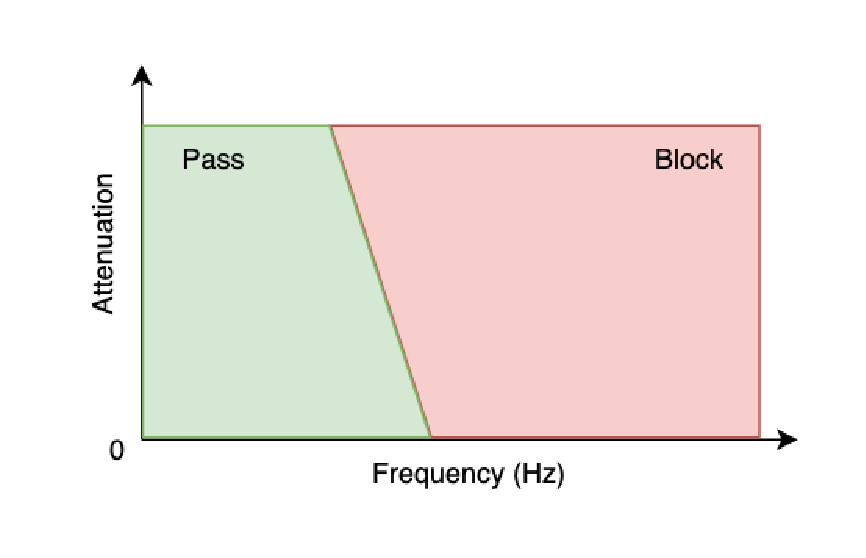
\includegraphics[width=\textwidth]{../images/pipeline/lowpass_filter.pdf}
        \captionsetup{width=\linewidth}
        \captionsetup{justification=centering}
        \caption{Low-pass filter.}
        \label{fig:processing_signals_filters_lowpass}
    \end{subfigure}
    \hfill
    \begin{subfigure}{0.45\textwidth}
        \centering
        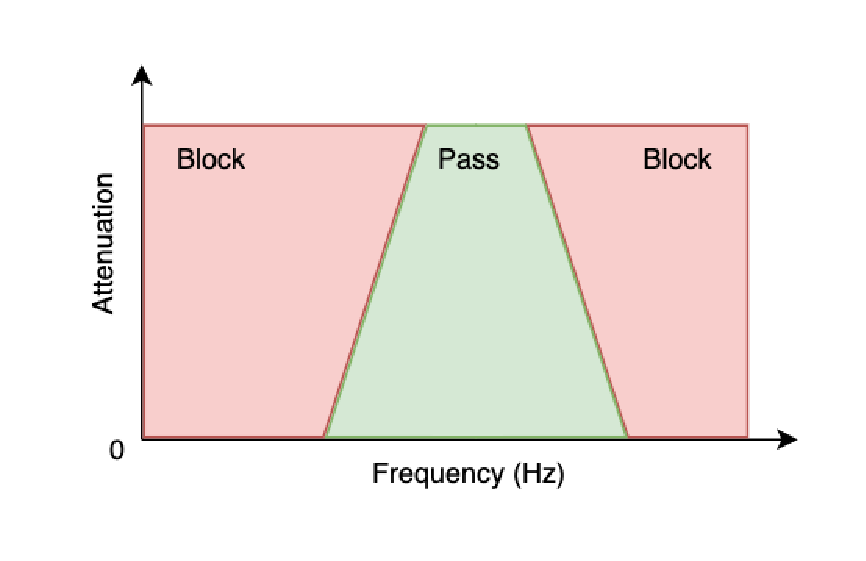
\includegraphics[width=\textwidth]{../images/pipeline/bandpass_filter.pdf}
        \captionsetup{width=\linewidth}
        \captionsetup{justification=centering}
        \caption{Band-pass filter.}
        \label{fig:processing_signals_filters_bandpass}
    \end{subfigure}
    \hfill
    \begin{subfigure}{0.45\textwidth}
        \centering
        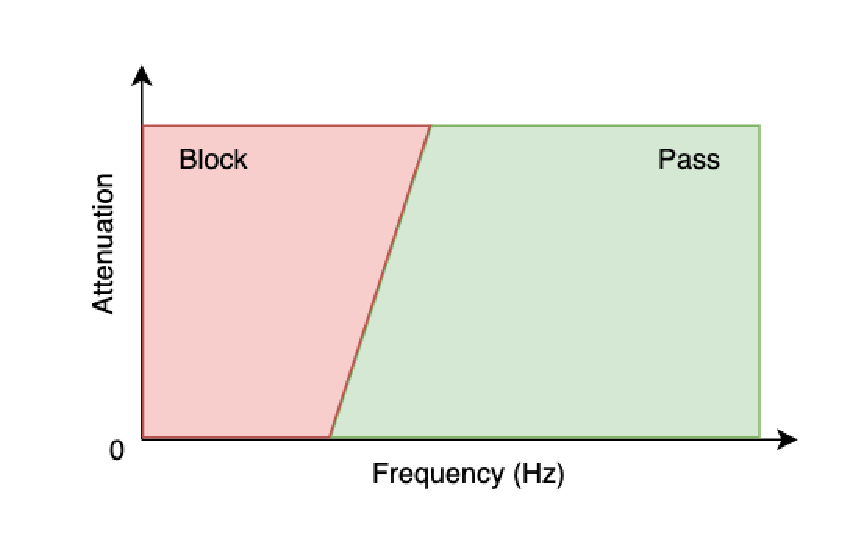
\includegraphics[width=\textwidth]{../images/pipeline/highpass_filter.pdf}
        \captionsetup{width=\linewidth}
        \captionsetup{justification=centering}
        \caption{High-pass filter.}
        \label{fig:processing_signals_filters_highpass}
    \end{subfigure}
    \hfill
    \begin{subfigure}{0.45\textwidth}
        \centering
        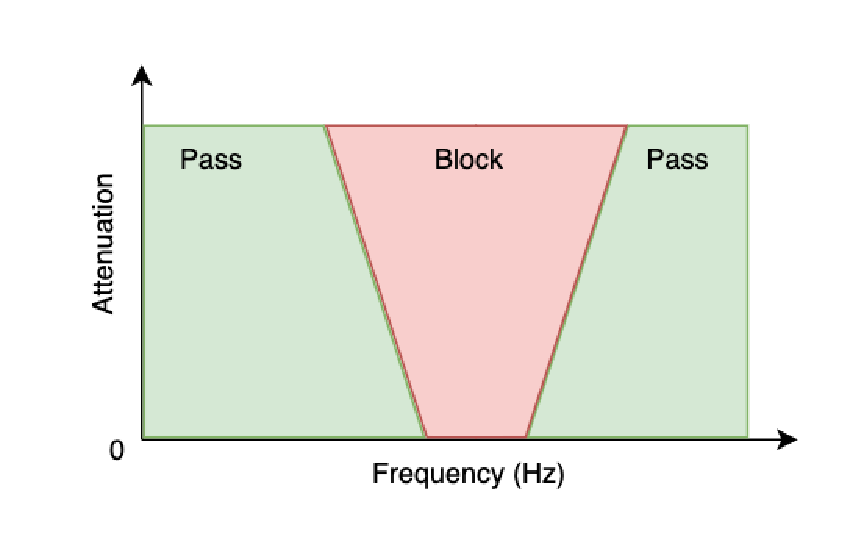
\includegraphics[width=\textwidth]{../images/pipeline/bandstop_filter.pdf}
        \captionsetup{width=\linewidth}
        \captionsetup{justification=centering}
        \caption{Band-stop filter.}
        \label{fig:processing_signals_filters_bandstop}
    \end{subfigure}
    \captionsetup{width=\linewidth}
    \captionsetup{justification=centering}
    \caption{Different types of filtering techniques.}
    \label{fig:processing_signals_filters}
\end{figure}

% | | | | | | | | | | | | |

\subsubsection{Baseline correction}
\label{subsubsec:processing_signals_general_pipeline_preprocessing_baseline_correction}

Another common preprocessing operation is baseline correction on a window.
Baseline correction consists of taking a baseline period and determining the mean voltage of each electrode's measurements during that baseline.
This baseline is most often one or more seconds before an event occurs.
This mean voltage is then subtracted from the remaining signal of each respective channel.
Doing this normalizes each window such that it has a centre closer to zero.
This can help in reducing the non-stationary problem and is used for the traditional two-step \gls{ml} experiments in this master thesis with a baseline period of one second before the event.

% | | | | | | | | | | | | |

\subsubsection{Channel and data downsampling or upsampling}
\label{subsubsec:processing_signals_general_pipeline_preprocessing_subsampling}

Another type of preprocessing is channel subsampling and augmentation through interpolation.
This consists of removing channels not of interest as discussed in Section \ref{subsec:biomedical_signals_working_with_eeg_anatomy} or adding augmented channels by clever interpolation or other approaches from the existing channels.
When a certain channel is known to be bad or artefacts described in Section \ref{subsec:biomedical_signals_working_with_eeg_artefacts} are detected, it may be replaced by an augmented channel during the artefact period as a way of resolving the artefact.
Likewise, if the sampling frequency of \gls{eeg} equipment is too high or low, data subsampling or upsampling may be performed.

% | | | | | | | | | | | | |

\subsubsection{Other preprocessing techniques and preprocessing ordering}
\label{subsubsec:processing_signals_general_pipeline_preprocessing_orders}

There exist many other preprocessing techniques for signals and \gls{mi} \gls{eeg} signals in particular but these fall outside the scope of this master thesis.
Preprocessing can happen in other places of the pipeline than the one shown in Figure \ref{fig:processing_signals_pipeline}, for example, channel subsampling reduces dimensionality and is thus often done as soon as possible to limit unneeded computational overhead.
It is important to note that multiple preprocessing steps may be performed in sequence.
This means that the output of a previous preprocessing step is used in the next and as such the ordering of preprocessing steps can be important depending on the techniques used in the sequence.
It is also important to note that certain preprocessing techniques which learn parameters from the training data should use the same parameters for the prediction pipeline, as redetermining them on the prediction data may alter the data in a way unknown by the already trained classifier later in the pipeline.
Whilst often not the case for preprocessing techniques, this is a subtility of great importance in feature engineering, the next step in the pipeline.



% - - - - - - - - - -
% Feature
% - - - - - - - - - -

% TODO: start here

\subsection{Feature engineering}
\label{subsec:processing_signals_general_pipeline_features}

% The CSP method performs feature extraction based on learned spatial filters.
% https://www.youtube.com/watch?v=zsOULC16USU

% Feature extraction: this final step is highly variable and depends on the exact context (sleep staging, Motor Imagery detection, epilepsy seizure detection, etc) in which the signal should be decoded. In general, DL models have been shown to perform better when the input is the raw (preprocessed) signal that is still represented as timeseries of samples for each signal channel. One of the most commonly used feature extraction methods is the Fourier transform, which allows to decompose a temporal signal (a sequence of signal readings over time) to a sum of sinuses of various frequencies. The Fourier transform transforms data from the time domain to the frequency domain. This transform is loss-less and invertible, which means that it does not destroy information. It allows the neural network to more easily focus on the existence of a particular frequency in a signal, instead of having to make sense of the entire (time-domain) signal.

% For a detailed review of possible feature extraction methods, we refer interested readers to Rashid et al (2020).

% ...Other feature engineering techniques zoals time-frequency domain

TODO

% - - - - - - - - - -
% Classification
% - - - - - - - - - -

\subsection{Classification}
\label{subsec:processing_signals_general_pipeline_classification}

TODO



% ---------------------------------------------- 
% ML AND DL TECHNIQUES
% ---------------------------------------------- 

\section{The role of machine learning and deep learning}
\label{sec:processing_signals_ml_and_dl}

% learning and prediction phase


% The dominance of CNN with regard to model choice can be attributed to the relative ease of use and the popularity of this architecture in other research fields that use DL. While RNN architectures have been successful in closely related fields such as speech recognition and natural language processing, they have only seen limited deployment in a biosignal decoding context. Typically, CNNs also have less trainable parameters which makes them less sensitive to small datasets and lower their computational requirements. Other architectures were investigated for biosignal decoding, but state-of-the-art research mostly focuses on CNN architectures (Buongiorno et al 2019, Roy et al 2019).

% nog een pro CNN en waarom wij focussen op CNN: The choice of DL model is highly dependent on the application requirements and how the data is preprocessed. CNNs can often work with raw data that is only cleaned in the preprocessing step, while other models will typically necessitate feature extraction before passing the input to the ANN (Schirrmeister et al 2017). Alternatively, RNNs are also used for biosignal decoding, but these architectures typically need more technical knowledge to deploy and evaluate. The literature review clearly shows that CNN is the most deployed model and that biosignal decoding models are typically rather shallow, which can be attributed to the limited availability of data.

% Neural networks e.v. lezen van review arnau

% dus wel RNN vermelden en uitleggen ma eigenlijk enkel zien naarr CNN based zoals de EEGnet en ShallowConvNet

% Designing a neural network requires experience, as there is no systematic approach. More information on neural networks and their architectures is presented in the appendix, section ‘Neural networks’.

% We refer readers interested in knowing more than what we present to books such as Goodfellow et al (2016) and Aggarwal (2018).

% - - - - - - - - - -
% Difference ML & DL
% - - - - - - - - - -

\subsection{Difference between traditional machine learning and deep learning}
\label{subsec:processing_signals_ml_and_dl_difference}

% nn_can_learn_from_raw
% % Conceptually, given enough layers and neurons, and the proper architecture, a neural network can learn any mapping from inputs to outputs (Sonoda and Murata 2017) (they are universal function approximators). This means that any method of acquiring a signal, and representing it as floatingpoint values will eventually allow the network to make sense of the inputs, and learn something. bci review arnau

TODO

% - - - - - - - - - -
% Common regular ML classifiers
% - - - - - - - - - -

\subsection{Machine learning paradigms}
\label{subsec:processing_signals_ml_and_dl_tyes_of_learning_supervision}

% Supervised, Semi-Supervised, Unsupervised, and Self-Supervised Learning

% The most common form of ML is supervised learning, in which we assume that the data is presented as a set of input-output pairs, a dataset, which we call labeled data, as each input is labeled with its corresponding output.

% The most common form of ML is supervised learning, in which we assume that the data is presented as a set of input-output pairs, a dataset, which we call labeled data, as each input is labeled with its corresponding output (Caruana and NiculescuMizil 2006). Alternatively, unsupervised learning techniques do not use outputs for learning, but rather learn the (unknown) structure of the data. Semi-supervised learning methods use both labeled and unlabeled data, usually to learn the structure of the training data to become able to generate more (artificial) training points (Aznan et al 2019), that are used for conventional supervised learning in a second learning phase. Self-supervised learning (Jing and Tian 2019) is a similar approach that is used to learn the relevant structure in EEG data by first learning an unsupervised pretext task, after which the model is further trained on the target task with labeled data (Banville et al 2020, Kostas et al 2021). The remainder of this review will focus on supervised learning methods.

% Semi-supervised learning methods use both labeled and unlabeled data. Their objective is to learn a supervised learning task, even in cases where only a small amount of training data is available. Usually, semi-supervised approaches learn the structure of the training data to become able to generate more (artificial) training points (Aznan et al 2019), that are used for conventional supervised learning in a second learning phase. Self-supervised learning (Jing and Tian 2019) is a similar approach which is currently gaining traction in the larger ML community. This technique was previously used to learn the relevant structure in EEG data by first learning an unsupervised pretext task, after which the model is further trained on the target task with labeled data (Banville et al 2020, Kostaset al 2021). The remainder of this review will focus on supervised learning methods.

% Therefore, low-confidence labelled data is often used in a semi-supervised fashion as explained by \citet{deep_learn_low_label}.

TODO

% - - - - - - - - - -
% Common traditional ML classifiers
% - - - - - - - - - -

\subsection{Common traditional machine learning classifiers}
\label{subsec:processing_signals_ml_and_dl_ml_classifiers}

% LDA
% SVM
% RF
% bekijk ml_strats_used_in_papers

% https://doi.org/10.1145/1143844.1143865 veergelijkt SVM en RF en andere

TODO

% - - - - - - - - - -
% Common DL classifiers
% - - - - - - - - - -

\subsection{Common deep learning classifiers}
\label{subsec:processing_signals_ml_and_dl_dl_classifiers}

% ANN (MLP fully connected -> wanneer DL en wanneer regular ML, uitleggen soms gezienals regular ML)
% CNN (conv layer, pooling layer)
% RNN (e.g. long term short term memory voor die layer)

% Veel al discussed in bci_opportunities_obstacles_motivating_examples_mi_models (BCIs)

% TODO: cnn bespreken a la: The most common type of DL neural networks at this time are the previously described CNNs (LeCun et al 1989). The subsequent application of convolutional layers results in a high-level representation of the input as stipulated by Goodfellow et al (2016). For example, in an object classification task, the network learns to extract primitive shapes from the raw input (a matrix of pixel values) in the first layer and then learns to extract objects from these primitive features in the next layer.
% en dus niet perse laatste layers voor classification maar vaak laatste layers terug mlps oid ipv puur convolutional layer

% In practice, neural networks can combine many layers of different kinds. It is not unusual to find neural networks that start with a few convolutional layers, to detect patterns independently of where they are in the input (such as edges in an image, or features in a 1D signal), then have one LSTM layer to be able to make sense of sequences of inputs, followed by a few feed-forward MLP-like layers to map what the LSTM layer learned to actual outputs. In the papers that we review in this article, great care is always given to explain and motivate the choice of neural architecture. Designing a neural network requires experience, as there is no systematic approach. We refer readers interested in knowing more than what we present here to books such as Goodfellow et al (2016) and Aggarwal (2018).


% bekijk ml_strats_used_in_papers

TODO

% ---------------------------------------------- 
% EVALUATING AND USING
% ---------------------------------------------- 
\section{Evaluating and using the classification pipeline}
\label{sec:processing_signals_evaluating_and_using}

% link back naar pipeline van cad

% duidelijk bespreken welk ding echt CS en welk ding eigenlijk derden

TODO

% - - - - - - - - - -
% trianing vs prediction
% - - - - - - - - - -

\subsection{Difference between training and prediction pipeline}
\label{subsec:processing_signals_evaluating_and_using_training_vs_prediction}

TODO

% - - - - - - - - - -
% offline vs online
% - - - - - - - - - -

\subsection{Difference between offline and online prediction}
\label{subsec:processing_signals_evaluating_and_using_offline_vs_online}

TODO

% - - - - - - - - - -
% calibration
% - - - - - - - - - -

\subsection{Calibrating a previously trained pipeline}
\label{subsec:processing_signals_evaluating_and_using_calibration}

TODO

% - - - - - - - - - -
% evaluting
% - - - - - - - - - -

\subsection{Evaluating the performance of the pipeline}
\label{subsec:processing_signals_evaluating_and_using_evaluation}

% CM
% acc
% loss
% f1
% ppv npv etc?
% CV 

TODO


% - - - - - - - - - -
% evaluting
% - - - - - - - - - -

\subsection{Hyperparameter tuning}
\label{subsec:processing_signals_evaluating_and_using_hyperparameter_tuning}

TODO

% ---------------------------------------------- 
% COMMON ISSUES
% ---------------------------------------------- 

\section{Common issues with MI classification pipelines}
\label{sec:processing_signals_common_issues}

TODO

% - - - - - - - - - -
% biased data
% - - - - - - - - - -

\subsection{Biased data}
\label{subsec:processing_signals_common_issues_bias}

TODO

% - - - - - - - - - -
% evaluation
% - - - - - - - - - -

\subsection{Incorrect or ambiguous evaluation}
\label{subsec:processing_signals_common_issues_generalisation}
% e.g. only look at a person we also used in training etc

TODO

% - - - - - - - - - -
% explainability and interpretability
% - - - - - - - - - -

\subsection{No explainability or interpretability}
\label{subsec:processing_signals_common_issues_exaplainable}

TODO

% TOODO
\Gls{dl} often requires significant processing power and time to train, impacting the affordability of \gls{bci} research.
This is especially true when working with many \gls{eeg} sensors and features, and thus a high dimensional setting. 
\Gls{dl} is often also used in a black-box principle.
This means that the trained system lacks explainability and interpretability.
% TODO explain both terms
Recent governmental reports have suggested that laws will be coming in place to require these properties \citep{eu_ai_blackbox_report, explainable_ai_policy}.

% - - - - - - - - - -
% overfitting
% - - - - - - - - - -

\subsection{Overfitting}
\label{subsec:processing_signals_common_issues_overfitting}

% To avoid over-fitting, Batch Normalization (Ioffe and Szegedy 2015) considers the input of every layer in a neural network, and normalizes it so that, in expectation, the inputs of every layer has a zero mean and a unit variance. Dropout (Srivastava et al 2014) does not modify the values that flow through a neural network, but instead randomly disables neurons every time the network is evaluated during training. Both these methods contribute to improving training speed and generalization of the network, and ensure that the model converges to an optimal loss. Both batch normalization (Tayeb et al 2019, Tam et al 2020) and dropout (Gautam et al 2020, Tortora et al 2020a) are often used in biosignal decoding papers, sometimes both at the same time. Other normalization techniques are possible, such as L1- normalization or clipping the gradients (Zhang et al 2019a), but they have been superseded by Batch Normalization and Dropout.

% generalization bespreken: With neural networks, the main avenue to increase generalization is to decrease over-fitting. Over-fitting happens when a neural network remembers exactly what training input should learn which training output, without having actually made sense of the data. The network achieves a training loss close to 0, but produces garbage output on the testing set. It is like a small child that learns how to read words, and remembers that card number 7 is pronounced ‘cat’, without actually looking at the word written on the card, or being able to read at all. Batch normalization (Ioffe and Szegedy 2015) considers the input of every layer in a neural network, and normalizes it so that, in expectation, the inputs of every layer has a zero mean and a unit variance. Intuitively, this normalization prevents ludicrously large or small values from appearing inside the network, which makes it ‘behave better’ or ‘be smoother’ (so, easier to train, and better at generalization). The actual mathematical way in which batch normalization works is however still unknown, with recent papers providing the first insights (Santurkar et al 2018). Dropout (Srivastava et al 2014) does not modify the values that flow through a neural network, but instead randomly disables neurons every time the network is evaluated during training. The main motivation behind Dropout is to avoid one particular neuron in the network to learn how to compensate (and thus cancel out) another particular neuron in the network. When neurons are constantly randomly disabled and re-enabled, they all have to learn independently from each other. More mathematically, Dropout leads to a neural network that is made of a different set of neurons every time it is evaluated. This leads to a large ensemble of ‘sub-networks’, all trained on different datapoints. Ensembles of function approximators such as this are known to help with generalization (Dietterich 2000). Both batch normalization (Tayeb et al 2019, Tam et al 2020) and Dropout (Gautam et al 2020, Tortora et al 2020a) are often used in biosignal decoding papers, sometimes both at the same time. Other normalization techniques are possible, such as L1- normalization or clipping the gradients (Zhang et al 2019a), but they have been superseded by Batch Normalization and Dropout.

% uit bci_review_arnau

TODO

% ---------------------------------------------- 
% CONCLUSIONS OF CHAPTER
% ---------------------------------------------- 
\section{Motivation for offline classification and chapter conclusions}
\label{sec:processing_signals_summary}
% TODO: summary of this chapter

% duidelijk bespreken classificiation echt CS terwijl die contorl vaak een andere (buiten interface ofc) ook link naar die paper division door ons
% bespreken paper division door ons zegt dat on classi model bruikbaar moet zijn maar dit nog net iets anders want offline, dus is eigenlijk nog further subdivision

TODO